% results_simulation.tex
\subsection{Simulation}
We have introduced this projected gamma distribution existing on $\mathcal{S}_{\infty}^{p-1}$.  As a
  means of evaluating how well we can recover a distribution under the proposed model, we have
  generated a series of datasets on $\mathcal{S}_{\infty}^{d-1}$, for $d$ ranging between 3 and 20.
  We generated each dataset from a mixture of projected Gammas, with the number of mixture components
  ranging between 3 and 12.  The generation procedure is detailed in Algorithm~\ref{algo:simulated}.
  \begin{algorithm}[H]
    \label{algo:simulated}
    % \setAlgoLined
    \For{$n_{\text{mix}}$ in $[3, 6, 9, 12]$}{
      Generate $n_{\text{mix}} \times 20$ shape Parameters $\alpha$\\
      Generate $n_{\text{mix}} \times 20$ Rate Parameters $\beta$\\
      Generate $500$ Mixture Component Identifiers $\delta$\\
      \For{$i$ in $1,\ldots,500$}{
        Generate ${\bf X}_i \sim \prod_{l = 1}^d\text{Ga}\left(X_{il}\mid\alpha_{\delta_i,l},\beta_{\delta_i, l}\right)$
        }
      \For{$n_{\text{col}}$ in $[3,6,12,20]$}{
        Project columns 1 to $n_{\text{col}}$ of ${\bf X}$ onto $\mathcal{S}_{\infty}^{n_{\text{col}} - 1}$ and save.
        }
    }
    \caption{Simulated Angular Dataset Generation Routine}
  \end{algorithm}
  The choice of generation routine for $\alpha = \alpha_0 + \alpha_1$ where
  $\alpha_0 \sim \text{Unif}(\alpha_0\mid 0,4)$, $\alpha_1\sim \text{Gamma}(\alpha_1\mid 1,1)$.
  The choice of generation routine for $\beta$ is $\beta\sim\text{Unif}(\beta\mid 0.25, 2.5)$.
  This choice was made to ensure that $\beta$ does not approach 0 in the generation routine.

\begin{figure}[h]
  \label{fig:simes}
  \caption{Simulation Energy Score versus Column Count, by Mixture Component Count}
  \centering
  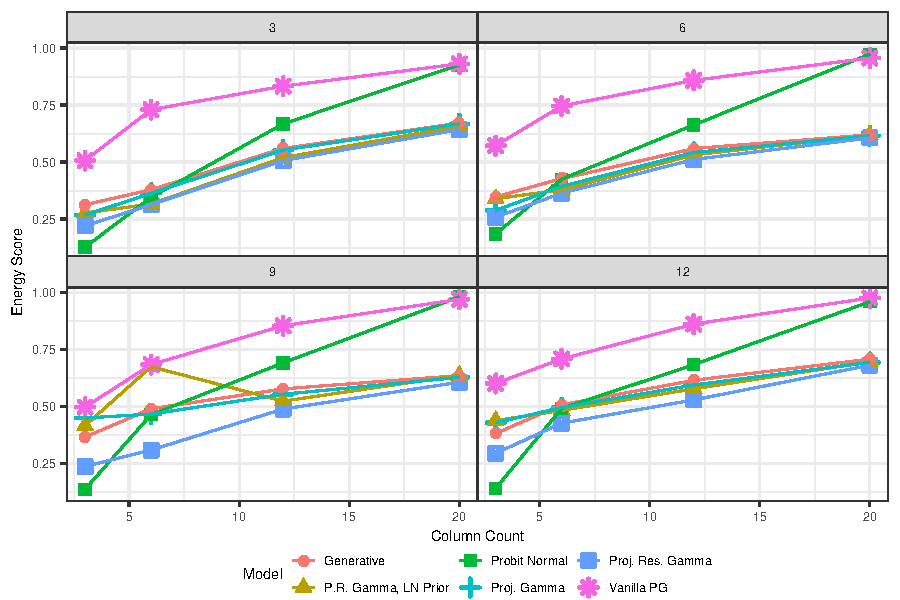
\includegraphics[width=0.8\textwidth]{./images/simulation_es}
\end{figure}

In Figure~\ref{fig:simes}, we fit DP Mixtures of the various models presented and plot the resulting
  energy score against the number of columns, grouped by the number of mixture components used in
  dataset generation.  The \emph{Generative} model refers to a dataset generated
  in the same manner, from the same parameters as was used to create the original dataset.  Against
  this generative dataset, we compare DP Mixtures of projected gamma, projected restricted gamma, and
  projected restricted gamma with a multivariate log-normal prior.  We observe that the projected
  restricted Gamma model dominates in most situations, but the difference between projected restricted
  Gamma and the other gamma-based models tends to shrink as the number of columns increases.
  Alternatively, that difference appears to grow as the number of mixture components increases.

\begin{figure}[h]
  \label{fig:simppl}
  \caption{Simulation Posterior Predictive Loss versus Column Count, by Mixture Component Count}
  \centering
  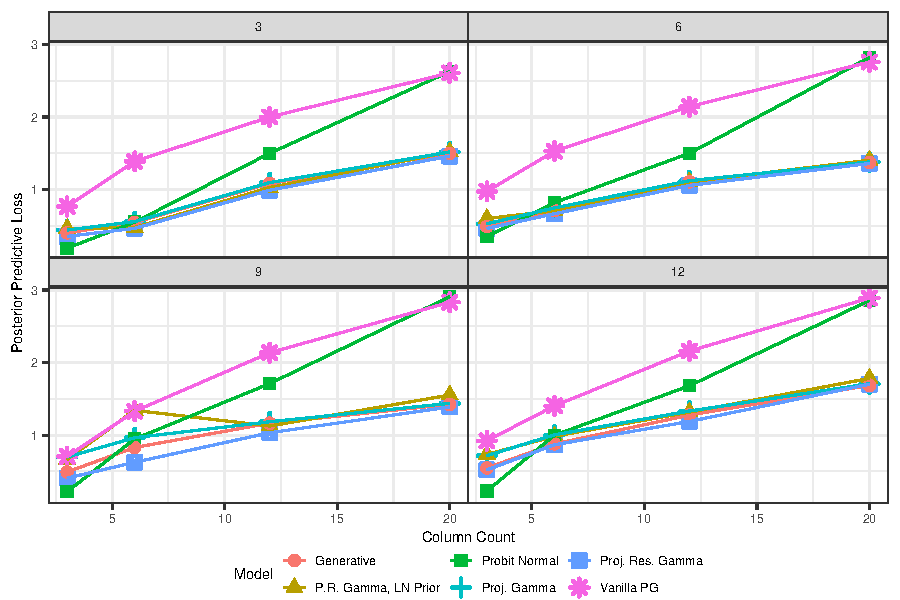
\includegraphics[width=0.8\textwidth]{./images/simulation_ppl}
\end{figure}

The posterior predictive loss criterion in Figure~\ref{fig:simppl} tells a similar story: the base
  model is inadequate for describing a mixture; and the DP mixture of projected restricted gammas
  performs the best of the presented models in most cases.  Interestingly, under both metrics we see
  the probit-normal model has the best performance when the number of columns is low.  That is
  unexpected behavior, as its performance very quickly degrades as the number of columns increases.

We frequently see all of the gamma-based mixture models accomplish a lower energy score than the generative
  distribution.  As \cite{nunez2019} noted, the projected Gamma model is very flexible and can generate
  multimodal distributions from a single mixture component.  When we allow a mixture model, we allow
  the possibility to break those modes into two different mixture components.  This will tend to
  result in a better energy score, as posterior predictive replicates for a given observation in a local
  model will tend to be concentrate in that local mode rather than being spread between multiple
  modes.  As for the dominance of projected restricted Gamma, By specifying $\beta_l := 1$ for all
  $l$, we are in effect forcing unimodal mixture components, which may not have been the case under
  the generative model.  As for whether this represents \emph{overfitting}, If we had reason to
  believe that the generative distribution for real data followed this form, then such a case could
  be made.  However, we are using projected Gamma as a parametric stand-in for an unknown distribution.
  In this sense, the argument for overfitting is less clear.

% EOF
